\section{Experimental Design}


\subsection{Motivation}
The motivation for the experiment was driven by four main questions:
\begin{enumerate}
\item Are participants performing better/more efficiently under any of the two conditions? (Accuracy, Interaction Time)
\label{question_1}
\item Are participants reporting that one of the two conditions was significantly more pleasant to use?
\label{question_2}
\item Is there a relationship between responses gathered for question \ref{question_1} and question \ref{question_2}? (E.g., was the system that is more efficient in processing the task also the one that is more pleasant to use?)
\item Does geometric complexity of interactive virtual objects have an impact on user performance?
\end{enumerate}

\subsection{VR-Scene Layout}
The layout for the VR environment was chosen to be minimal. Participants start out in a square room which comprises the full scene and all objects necessary for the experiment.

Objects in the room are:
\begin{itemize}
\item 4 \textit{tables}, one along each wall in the room
\item 6 \textit{interactive objects} the participants can manipulate
\item 6 \textit{translucent shapes} to indicate target position and orientation of interactive objects
\item 1 interactive \textit{exit sign} for ending the experiment
\end{itemize}

Both interactive and translucent objects are members of three different object groups:
\textit{Cubes}, \textit{5-pointed stars} and \textit{6-pointed stars}. From each group two interactive and two translucent instances, one large and one small respectively, are included.

Interactive objects are initially placed together on one table.
Orientation and position of the interactive objects is arbitrary, but the same for every participant (see figure \ref{figure_object_placement}).
This was done to avoid inducing preference for processing of objects in any specific order.
Participants start out in the center of the room, facing the table that holds the interactive objects so that it is the first thing they see in the beginning of their experimental run.

The remaining three tables can then be found to their left, right and behind them (see figure \ref{figure_experiment_layout}). On each of these three tables, the translucent shapes of objects of one specific kind can be found.

\begin{figure}
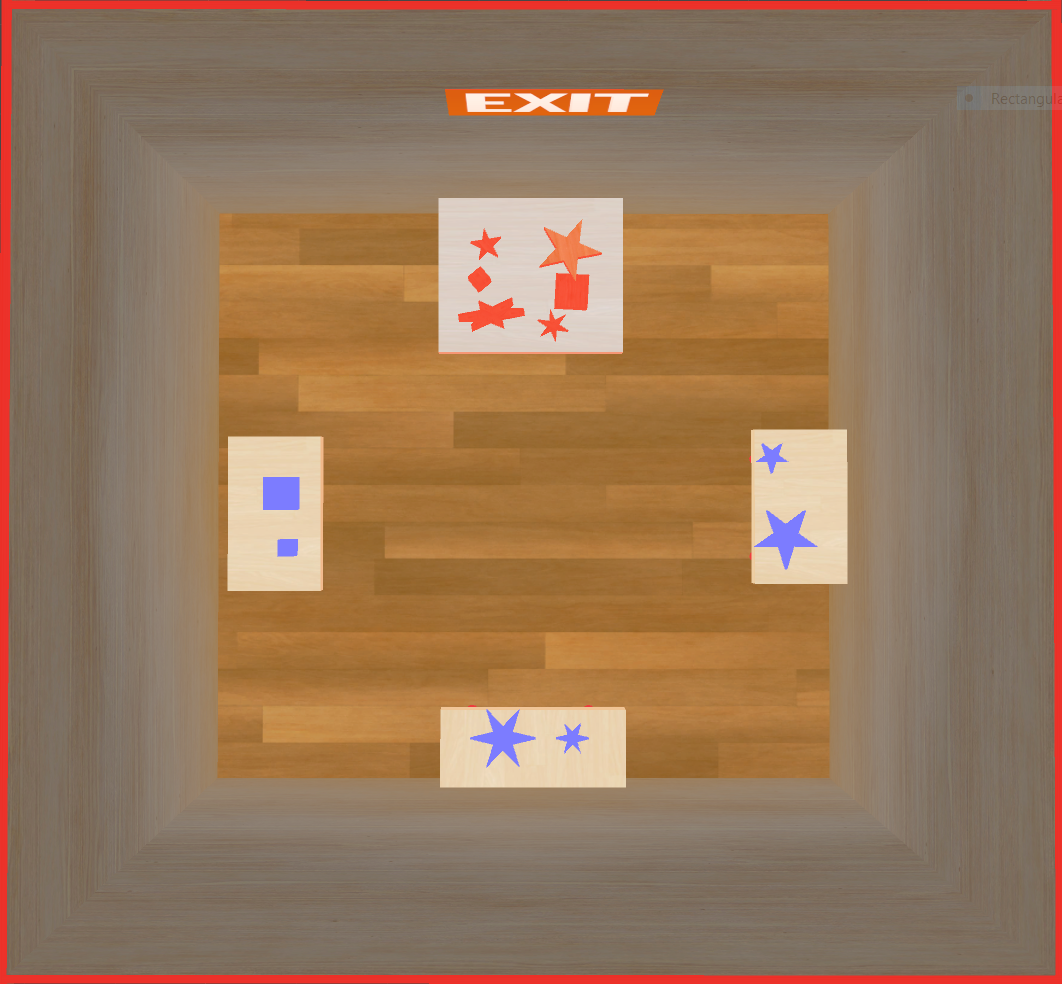
\includegraphics[width=0.48\textwidth]{figures/map_top_mipmap.PNG}
\caption{
\textsf{Top-down view of the virtual scene. Object's are colored in for this depiction only to indicate their purpose. Red: Interactive objects; Blue: Translucent objects marking target positions; The 'EXIT' button to end the experiment run can be seen at the top of the figure.}
}
\label{figure_experiment_layout}
\end{figure}
\begin{figure}
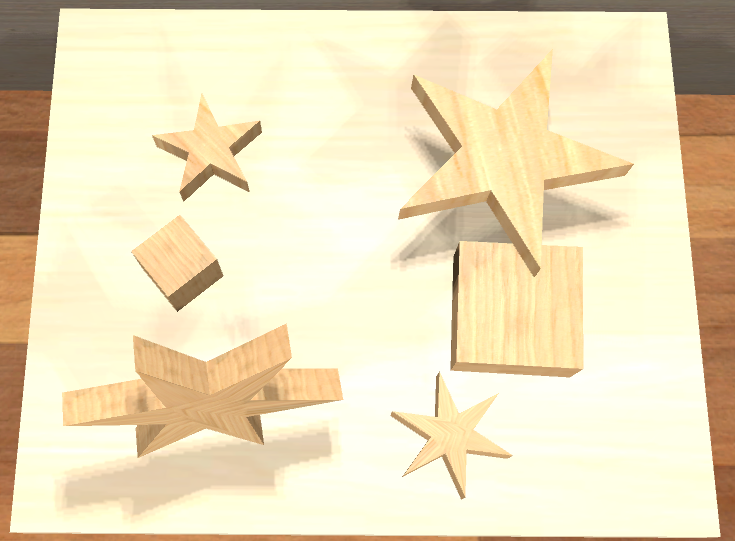
\includegraphics[width=0.48\textwidth]{figures/object_placement.PNG}
\caption{
\textsf{Close up view of the initial object placements. This placement was chosen arbitrarily but is the same for all participants.}
}
\label{figure_object_placement}
\end{figure}


\subsection{User Task \& Measurements}
The participant is confronted with the task of placing interactive objects in a specific position and orientation using the interaction methods available to them under given interaction mode.
As mentioned before, the precise target position and orientation is indicated by translucent objects matching the interactive object in size and shape.

The experiment is conducted in two separate runs.
During each of the runs participants are restricted to one of the two interaction modes (Hand Gesture Recognition / Touch Gesture Recognition). During placement of each interactive object a number of parameters are then recorded:
\begin{itemize}
\item total rotation applied (in degrees)
\item rotational deviation from target rotation (in degrees around each axis)
\item positional deviation from target position
\item number of selections of the object
\item time spend on handling the object
\end{itemize}
After each round the participants where required to fill out questionnaires for:
\begin{itemize}
\item usability of the performed interaction method (System Usability Scale).
\item task work load (NASA-Task Load Index)
\end{itemize}


\subsection{Typical Course of the Experiment}
Before the start of the simulation participants are introduced to the task and possible interaction methods verbally.
Usually, if the participant didn't have any prior experience with VR-simulations they would take a minute just to make themselves comfortable with the VIVE-headset and orientation in the environment.
After the introduction to the modality-specific gestures the participant then begins the task.

Subsequent to completing the task under the first modality participants could take a short break.
Then an introduction to the other modality would be given, explaining the second set of modality-specific gestures.
Throughout the course of the experiment the moderators would not intervene.
Participants were told to ask whenever they might forget how to perform a specific interaction or the precise task so they could be reminded.